% !TeX TXS-program:compile = txs:///pdflatex/[--shell-escape]
\documentclass[10pt,landscape,a4paper]{article}
\usepackage[table]{xcolor}
\usepackage[normalem]{ulem}
\usepackage{tikz}
\usetikzlibrary{shapes,positioning,arrows,fit,calc,graphs,graphs.standard}
\usepackage[nosf]{kpfonts}
\usepackage[t1]{sourcesanspro}
\usepackage{multicol}
\usepackage{wrapfig}
\usepackage[top=1mm,bottom=1mm,left=1mm,right=1mm]{geometry}
\usepackage[framemethod=tikz]{mdframed}
\usepackage{microtype}
\usepackage{tabularx}
\usepackage{hhline}
\usepackage{makecell}
\usepackage{mathtools}
\usepackage{subfig}
\usepackage{listings}
\usepackage{soul}
\usepackage{amsmath,amsthm,amsfonts,amssymb}

\graphicspath{ {./img/} }

\DeclarePairedDelimiter{\ceil}{\lceil}{\rceil}

\definecolor{myblue}{cmyk}{1,.72,0,.38}

\pgfdeclarelayer{background}
\pgfsetlayers{background,main}

\renewcommand{\baselinestretch}{.8}
\pagestyle{empty}

\let\counterwithout\relax
\let\counterwithin\relax
\usepackage{chngcntr}
\usepackage{verbatim}
\usepackage{etoolbox}
\makeatletter
\preto{\@verbatim}{\topsep=0pt \partopsep=0pt }
\makeatother

\counterwithin*{equation}{section}
\counterwithin*{equation}{subsection}
\usepackage{enumitem}
\newlist{legal}{enumerate}{10}
\setlist[legal]{label*=\arabic*.,leftmargin=3mm}
\setlist[itemize]{leftmargin=3mm}
\setlist[enumerate]{leftmargin=3.5mm}
\setlist{nosep}
\usepackage{minted}

\newenvironment{descitemize} % a mixture of description and itemize
{\begin{description}[leftmargin=*,before=\let\makelabel\descitemlabel]}
	{\end{description}}
\newcommand{\descitemlabel}[1]{%
	\textbullet\ \textbf{#1}%
}
\makeatletter

\renewcommand{\section}{\@startsection{section}{1}{0mm}%
	{.2ex}%
	{.2ex}%x
	{\color{myblue}\sffamily\small\bfseries}}
\renewcommand{\subsection}{\@startsection{subsection}{1}{0mm}%
	{.2ex}%
	{.2ex}%x
	{\sffamily\bfseries}}
\renewcommand{\subsubsection}{\@startsection{subsubsection}{1}{0mm}%
	{.2ex}%
	{.2ex}%x
	{\rmfamily\bfseries}}

\makeatother
\setlength{\parindent}{0pt}
\setminted{tabsize=2, breaklines}
% Remove belowskip of minted
\setlength\partopsep{-\topsep}

\newcolumntype{a}{>{\hsize=1.5\hsize}X}
\newcolumntype{b}{>{\hsize=.25\hsize}X}

\setlength\columnsep{10pt}
\setlength\columnseprule{0pt}
\begin{document}
\abovedisplayskip=0pt
\abovedisplayshortskip=0pt
\belowdisplayskip=0pt
\belowdisplayshortskip=0pt
\scriptsize
%\tiny
\begin{multicols*}{4}
  \raggedcolumns
  \section{Introduction to AI}
  \subsection{What is AI}
  \begin{itemize}
  	\item Intelligent mechanisms that solve problems to help humans
  	\begin{itemize}
  		\item concerned with human thinking
  		\item assessed based on generality (more dynamic solutions that is able to deal with many cases) and performance (perform at least as well as humans)
  	\end{itemize}
  \end{itemize}
  \subsection{Kinds of AI}
  \begin{itemize}
  	\item Strong AI
  	\begin{itemize}
  		\item General problem solver $\rightarrow$ very dynamic program that solves many problems
  	\end{itemize}
  	\item Weak/Narrow AI
  	\begin{itemize}
  		\item Less dynamic program $\rightarrow$ typically solves 1 problem, easier to formalize
  	\end{itemize}
  \end{itemize}
  \subsection{Rational Agent}
  \begin{itemize}
    \item An agent is an entity that perceives its \textbf{environment} through \textbf{sensors} (what is captured about environment) and acts through \textbf{actuators} (how agent affect change in environment)
    \item An agent's \textbf{percept sequence} is the complete history of everything the agent has ever perceived.
    \item What is rational depends on: (1) quantifiable performance measure that defines success, (2) prior knowledge of the env, (3) actions available, (4) percept sequence to date.
    \item For each possible \textcolor{red}{percept sequence}, a Rational Agent should select an action that is expected to maximize its performance measure, given the evidence provided by the percept sequence and whatever built-in knowledge the agent has.
  \end{itemize}
  \begin{center}
   	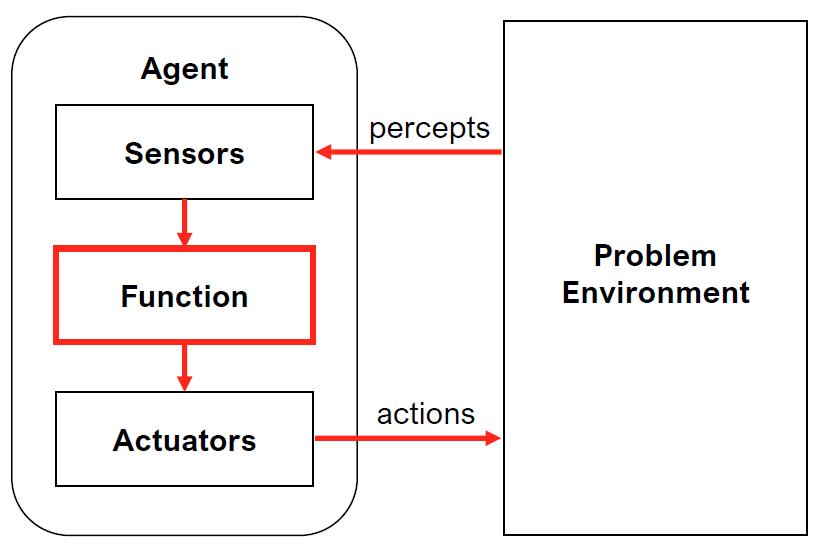
\includegraphics[width=0.6\columnwidth]{agent_framework}
  \end{center}
  \subsection{AI as Graph Search}
  \begin{itemize}
  	\item Percept $\rightarrow$ state/vertex
  	\item Desired states $\rightarrow$ goals
  	\item Actions $\rightarrow$ edges
  	\item Search space $\rightarrow$ graphs
  	\item Solved using graph search algorithms
  \end{itemize}
  \subsection{Environment Properties}
  \begin{itemize}
    \item \textbf{Fully observable} vs \textbf{Partially observable}: Partially observable agent does not have access to all information (e.g. fully observable maze VS slowly expanding maze based on actions taken). Requires dealing with \textbf{uncertainty} i.e. backtracking algos 
    \item \textbf{Deterministic} vs \textbf{Stochastic}: if the next state of the env is completely determined by the current state and the action executed \textbf{VS} otherwise. (A fully observable environment that has randomness with action is stochastic) (e.g. Sudoku VS Poker)
    \item \textbf{Episodic} vs \textbf{Sequential}: actions only impact current state \textbf{VS} action impact future decisions
    \item \textbf{Discrete} vs \textbf{Continuous}: in terms of state of env, time, percepts and actions (tend to discretize continuous environments)
    \item \textbf{Single agent} vs \textbf{Multi-agent}: whether there are any other agent in the environment whose actions directly influence the performance of this agent, multi-agent further divided into \textbf{competitive} and \textbf{cooperative}
    \item \textbf{Static} vs \textbf{Dynamic}: if the environment is unchanged while an agent is deliberating \textbf{VS} otherwise
  \end{itemize}
  \subsection{Agent Types, in increasing generality}
  \begin{itemize}
    \item \textbf{Simple Reflex Agent}: narrow agents, follows set of rules (if-else statements) to make decision, direct mapping of percepts to actions, mostly domain specific, impractical with large search space (requires iterating through all cases)
    \item \textbf{Model-based Reflex Agents}: Makes decision based on internalized model (typically logical agents or bayesian networks)
    \item \textbf{Goal-based/Utility-Based Agent}: given state and available actions, determines a sequence of actions to reach goal/maximize utility (typically solved using search algo, local search, CSP or adversarial search)
    \item \textbf{Learning Agent}: Agents that learn how to optimize performance
  \end{itemize}

  \section{Solving Problems by Searching}
  \subsection{Path Planning Problem Properties}
  \begin{itemize}
  	\item Environment assumed to be fully observable, deterministic, discrete and episodic (assume that we can see the whole problem, plan a path and then execute it)
  	\item Plan is formed sequentially, each action in the plan impacts the next action in the plan, one plan (path) is independent from another plan
  \end{itemize}
  \subsection{Problem Formulation}
  \textbf{State} (abstract data types that describes the environment), \textbf{Actions} (function that returns set of actions possible given a particular state), \textbf{Transition Models} (description of each action), \textbf{Goal Test} (determines whether a state is a goal state), \textbf{Path/Action Cost} (assigns a numeric cost to each path)
  \textcolor{red}{A \textbf{node} includes state, parent node, action, and path cost, depth}
  \subsection{Evaluation criteria}
  \begin{itemize}
    \item \textbf{Completeness}: always find solution if one exists and correctly report failure when there is no solution
    \item \textbf{Optimality}: finding a least-cost solution
    \item \textbf{Time complexity}: no of nodes generated
    \item \textbf{Space complexity}: max. no of nodes in memory
  \end{itemize}
  \subsection{Problem parameters}
  \begin{itemize}
    \item $b$: max. no of successors of any node (branching factor)
    \item $d$: depth of shallowest goal node
    \item $m$: max. depth of search tree
  \end{itemize}
  \subsection{Uninformed Search}
  \textbf{Uninformed Search Strategies}

  \begin{tabular}{l|l|l|l|l|l}
    \textbf{Property} & \textbf{BFS} & \textbf{UCS}                                             & \textbf{DFS} & \textbf{DLS} & \textbf{IDS} \\ \hline
    \textbf{Complete} & Yes*         & Yes**                                                    & No***        & No           & Yes*         \\
    \textbf{Optimal}  & No*          & Yes                                                      & No           & No           & No*          \\
    \textbf{Time}     & $O(b^d)$    & $O(b^{1+\left\lfloor\frac{C^*}{\epsilon}\right\rfloor})$ & $O(b^m)$     & $O(b^l)$     & $O(b^d)$     \\
    \textbf{Space}    & $O(b^d)$     & $O(b^{1+\left\lfloor\frac{C^*}{\epsilon}\right\rfloor})$ & $O(bm)$      & $O(bl)$      & $O(bd)$      \\
  \end{tabular}
  
  *: BFS, IDS -- complete if $b$/state space is finite or if there is a solution, optimal if step costs are identical

  **: UCS is complete if $b$ is finite and action cost $> \epsilon > 0$

  ***: DFS is complete only on finite depth \& branching factor graphs
  
  $C^*$ is the optimal cost

  \subsubsection{Breadth-First Search (BFS)}
  Expand shallowest unexpanded node, frontier is FIFO. Takes $O(b^{d+1})$ space if using late goal test. Typically use \textbf{Graph Search}
  \subsubsection{Uniform-Cost Search (UCS)}
  Expand least-path-cost unexpanded node, frontier is PQ by path cost. Equivalent to BFS if all step costs are equal
  \subsubsection{Depth-First Search (DFS)}
  \begin{itemize}
    \item Expand deepest unexpanded node, frontier is LIFO.
    \item \textbf{Backtraking Search}, space can be $O(m)$ if successor is expanded one at a time (partially expanded node remembers which successor to generate next)
    \item Typically use \textbf{Tree Search}
  \end{itemize}
  \subsubsection{Depth-Limited Search (DLS)}
  Run DFS with depth limit $l$, to solve the infinite-path problem
  \subsubsection{Iterative Deepening Search (IDS)}
  \begin{itemize}
    \item  Perform DLS with increasing depth limit.
    \item Preferred if search space is large and depth of solution is not known
    \item Properties of completeness from BFS with space complexity of DFS, disadvantage of reruning top levels many times
  \end{itemize}
  \subsection{Tree vs Graph Search}
  \textbf{Graph search} could contain cycles \& redundant paths and requires a \textbf{visited} hashmap to prevent revisits
  
  \textbf{Tree search} on the other hand allows revisits 
  \subsubsection{Graph Search Versions}
  \begin{tabular}{c c}
  	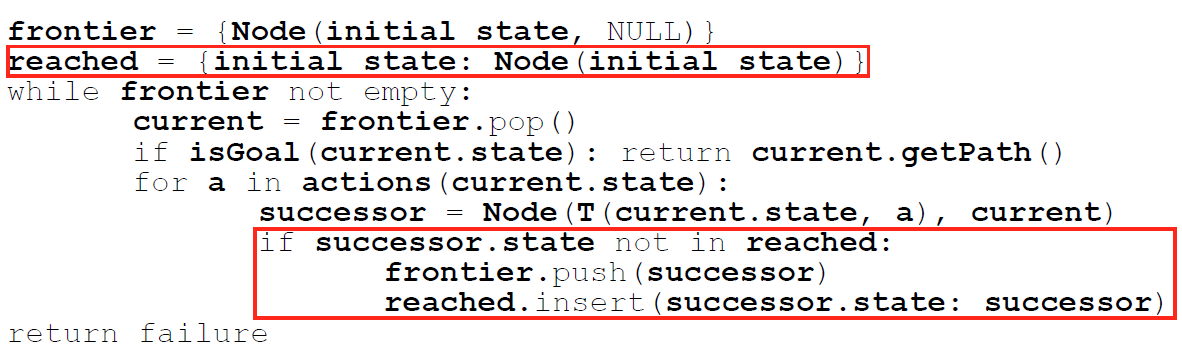
\includegraphics[width=0.5\linewidth]{graph_v1}
  	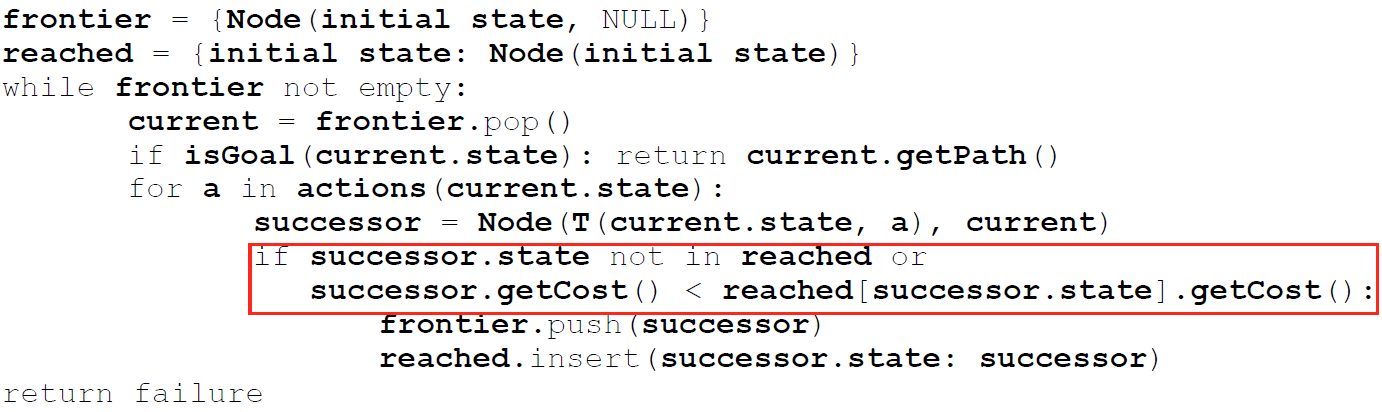
\includegraphics[width=0.5\linewidth]{graph_v2}
  \end{tabular}
  Graph search V1 ensures nodes are not revisited which \textcolor{red}{could omit optimal paths}
  
  Graph search V2 solves that by allowing revisits provided cost is lower
  \subsubsection{Graph Search Properties}
  \begin{itemize}
  	\item Time and space complexity are both $O(|V|+|E|)$
  \end{itemize}
  \subsection{Informed Search}
  \textbf{Informed (Heuristic Search Strategies)}
  
  Idea is to use domain knowledge to determine cost required to go from particular state to nearest goal which reduces search space
  \subsubsection{Greedy best-first search}
  \begin{itemize}
    \item $f(n) = h(n) = $ estimated cost of cheapest path from $n$ to goal
    \item Expands nodes that appear to be closest to the goal
    \item \textbf{Incomplete} $\rightarrow$ can get stuck in loop between nodes where $h$ values are lowest, \textbf{Non-optimal} under both tree and graph search, \textbf{Time} $O(b^m)$, \textbf{Space} $O(b^m)$
  \end{itemize}
  \begin{center}
  	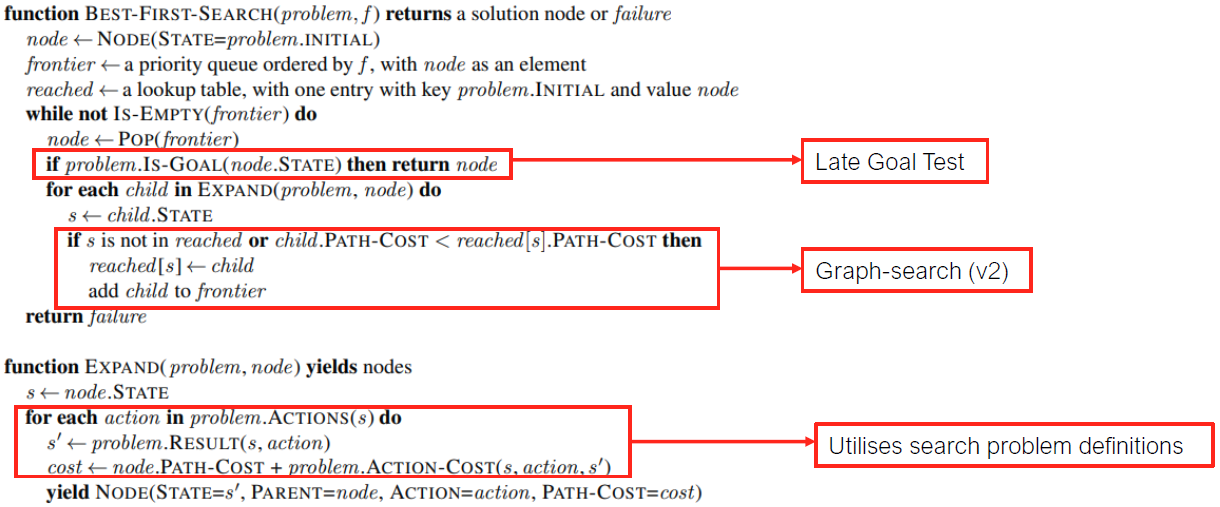
\includegraphics[width=0.7\columnwidth]{best-first}
  \end{center}
  \subsubsection{A* Search}
  \begin{itemize}
    \item $f(n) = g(n) + h(n)$, $g(n) = $ path cost from start node to node $n$
    \item Avoids expanding paths that are already expensive
    \item \textbf{Admissible Heuristic} never overestimates the cost to reach the goal: $\forall n, h(n) \leq h^*(n)$ where $h^*(n) = $ true cost
    \begin{itemize}
    	\item Consequence: all paths with actual costs less than $P$ must be searched
    \end{itemize}
    \item \textbf{Consistent Heuristic}: $h(n) \leq c(n, n') + h(n')$, will make $f(n)$ monotonically increasing along a path
    \item \textcolor{red}{Consistency $\implies$ Admissibility}
    \item $h(n)$ is \textbf{admissible}:
    \begin{itemize}
    	\item Optimal under \textbf{Tree Search} and \textbf{Graph Search V2}
    	\item Non-optimal under \textbf{Graph Search V1}
    \end{itemize}
    \item $h(n)$ is \textbf{consistent}: 
    \begin{itemize}
    	\item Optimal under \textbf{Tree Search}, \textbf{Graph Search V2 and V3} (insert into visited when popped)
    	\item Non-optimal under \textbf{Graph Search V1}
    \end{itemize}
    \item \textbf{Complete} if $b$ \& $m$ finite OR has a solution and all action cost $> \epsilon > 0$, \textbf{Optimal}, \textbf{Time} $O^{h^*(s_0) - h(s_0)}$ where $h^*(s_0)$ is the actual cost of getting from root to goal, \textbf{Space} $O(b^m)$
    \item \textbf{Dominant heuristic}: if $\forall n, h_2(n) \geq h_1(n)$ then $h_2$ \textbf{dominates} $h_1$
    \item More dominant heuristics incur lower search cost
  \end{itemize}

  \section{Goal Search}
  \begin{itemize}
    \item Path to goal is irrelevant, the goal state itself is the solution.
    \item Advantages: (1) use very little $O(b)$/constant memory, (2) can find reasonable solns in large/infinite continuous state spaces
    \item Useful for \textbf{pure optimization problems}: objective is to find the best state according to an \textbf{objective function}. e.g. Vertex cover, TSP, Boolean Satisfiability Problem (SAT), Timetabling/scheduling
  \end{itemize}
  \subsection{Hill-climbing Algorithms}
  \subsubsection{Problem Formulation}
  \begin{itemize}
  	\item Start with \textbf{complete} state i.e. no partial state (removes build up stage and start checking on 1st iteration)
  	\item Each state is a possible solution
  \end{itemize}
  \subsubsection{Steepest Ascent - Greedy}
  \begin{itemize}
    \item Start with random initial state, in each iteration find successor that improves on current state
    \item Requires \textbf{actions} and \textbf{transition} to determine successors
    \item Requires some heuristic to give value to each state e.g. $f(n)=-h(n)$ and find maxima
    \item Algorithm \textbf{can get stuck at local maxima} and return non-goal state
    \item Problems arises if met with \textbf{shoulders/plateau, local maxima or ridge}
  \end{itemize}
  \begin{center}
  	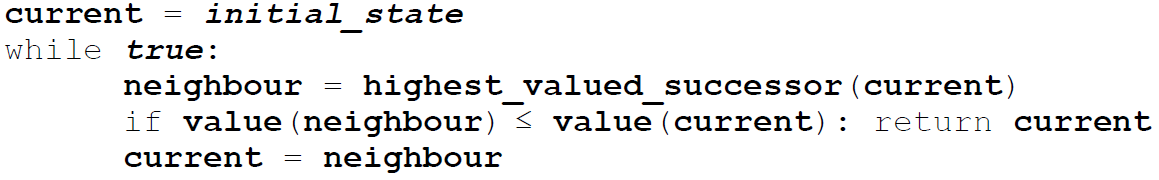
\includegraphics[width=0.75\columnwidth]{hill-climb}
  \end{center}
  \subsubsection{Stochastic Hill Climbing}
  \begin{itemize}
  	\item Instead of choosing highest-valued-successor in each step, \textbf{choose randomly among states with better values} instead
  	\item Idea is to make the choosing of next state less deterministic to give to algo more chance of finding global maxima
  	\item Takes longer but could lead to better solutions
  \end{itemize}
  \subsubsection{First-choice Hill Climbing}
  \begin{itemize}
  	\item Handles high branching factor by randomly generating successors until one with better value is found
  	\item Possible to achieve $O(1)$ space with this 
  \end{itemize}
  \subsubsection{Sideways Move}
  \begin{itemize}
  	\item Replace the $\leq$ sign in steepest ascent with $<$ 
  	\item Allows algo to traverse shoulders/plateaus
  \end{itemize}
  \subsubsection{Random-restart}
  \begin{itemize}
  	\item Adds outer loop which randomly pick new starting state and keep attempting restarts until solution is found (up to a certain threshold)
  	\item Also allows for sideways move
  \end{itemize}
  \begin{center}
  	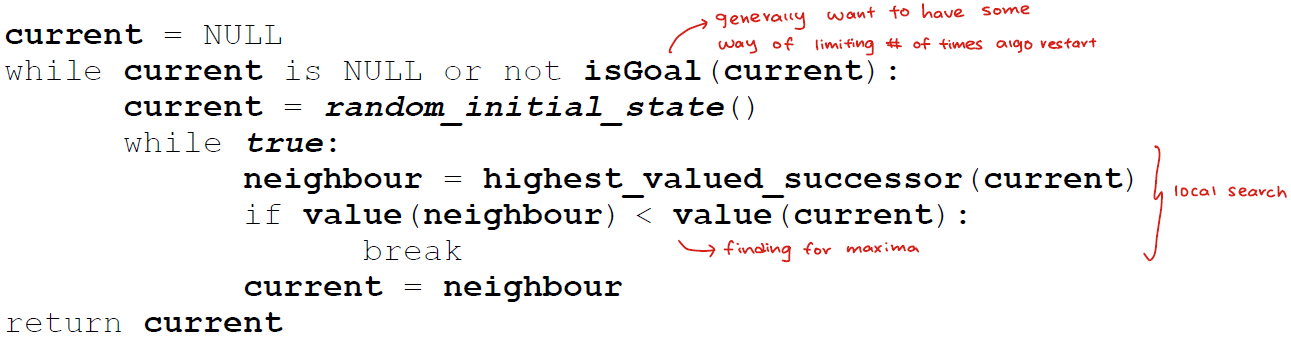
\includegraphics[width=0.8\columnwidth]{random-restart}
  \end{center}
  \subsection{Analysis of Hill Climb}
  \begin{center}
  	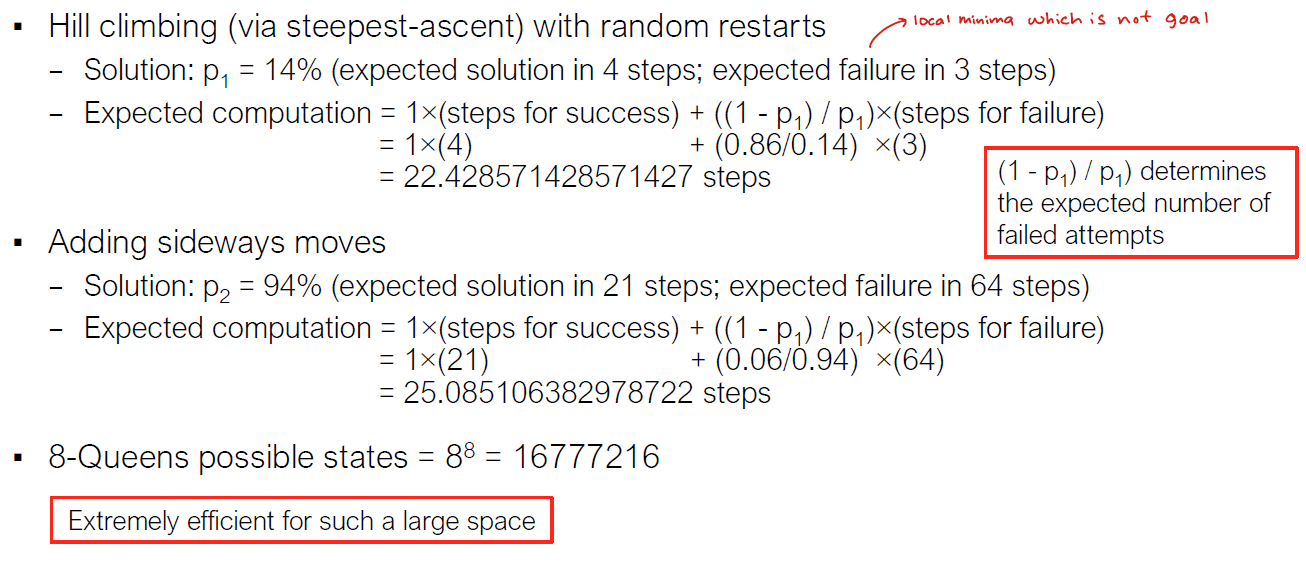
\includegraphics[width=0.9\columnwidth]{hill-climb-analysis}
  \end{center}
  \subsection{Local Beam Search}
  \begin{itemize}
  	\item Stores $k$ states instead of 1
  	\item Algo begins with $k$ random restarts which generates successors for all $k$ states
  	\item Next iteration will repeat the above step with best $k$ among ALL generated successors found (unless goal is found)
  	\item Better than $k$ parallel random restarts, Since best $k$ among ALL successors taken (not best from each set of successors, $k$ times)
  	\item Also has a stochastic variant to increase probability of escaping from local maxima
  \end{itemize}
  \section{Search Problem Representation}
  \begin{enumerate}
  	\item State Representation
  	\begin{itemize}
  		\item State how the problem is represented e.g. $m\times n$ grid
  		\item State values that each cell/state can take e.g. "1" means action performed, "0" means valid, "X" means invalid
  		\item How the position is encoded e.g. (x, y)
  	\end{itemize}
  	\item Initial State
  	\begin{itemize}
  		\item How each cell/state is initially labeled i.e. how do you determine what is initially labeled "X" or "0" or "1"
  		\item Starting position
  	\end{itemize}
  	\item Actions
  	\begin{itemize}
  		\item Movements e.g. Up down left right
  		\item Possible actions to take e.g. clean cell, eat cell etc.
  	\end{itemize}
  	\item Transition
  	\begin{itemize}
  		\item How to update cells
  	\end{itemize}
  	\item Step cost
  	\item Goal test
  \end{enumerate}
  \section{Local Search Problem Representation}
  \begin{itemize}
  	\item Initial state
  	\begin{itemize}
  		\item How do you get the first "complete" state
  		\item What heuristic is being used?
  		\item How do we assign a value to the initial state?
  	\end{itemize}
  	\item Finding next state
  	\begin{itemize}
  		\item How do we transition from one state to another? What actions are taken?
  	\end{itemize}
  	\item Stopping State
  	\begin{itemize}
  		\item What happens if $val(next_state)\leq val(curr_state)$?
  		\item What happens if $val(next_state) > val(curr_state)$?
  	\end{itemize}
  \end{itemize}
  \section{Proofs}
  \subsection{Why is UCS optimal?}
  \begin{center}
  	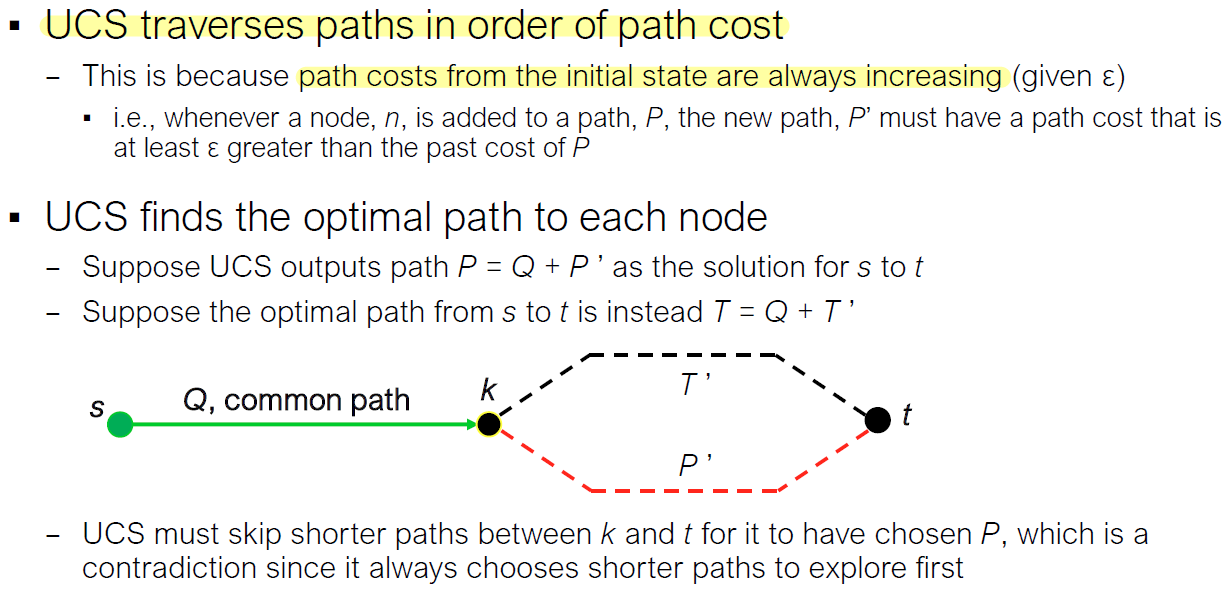
\includegraphics[width=0.7\columnwidth]{ucs-optimality}
  \end{center}
  \subsection{Why is A* optimal?}
  \begin{center}
  	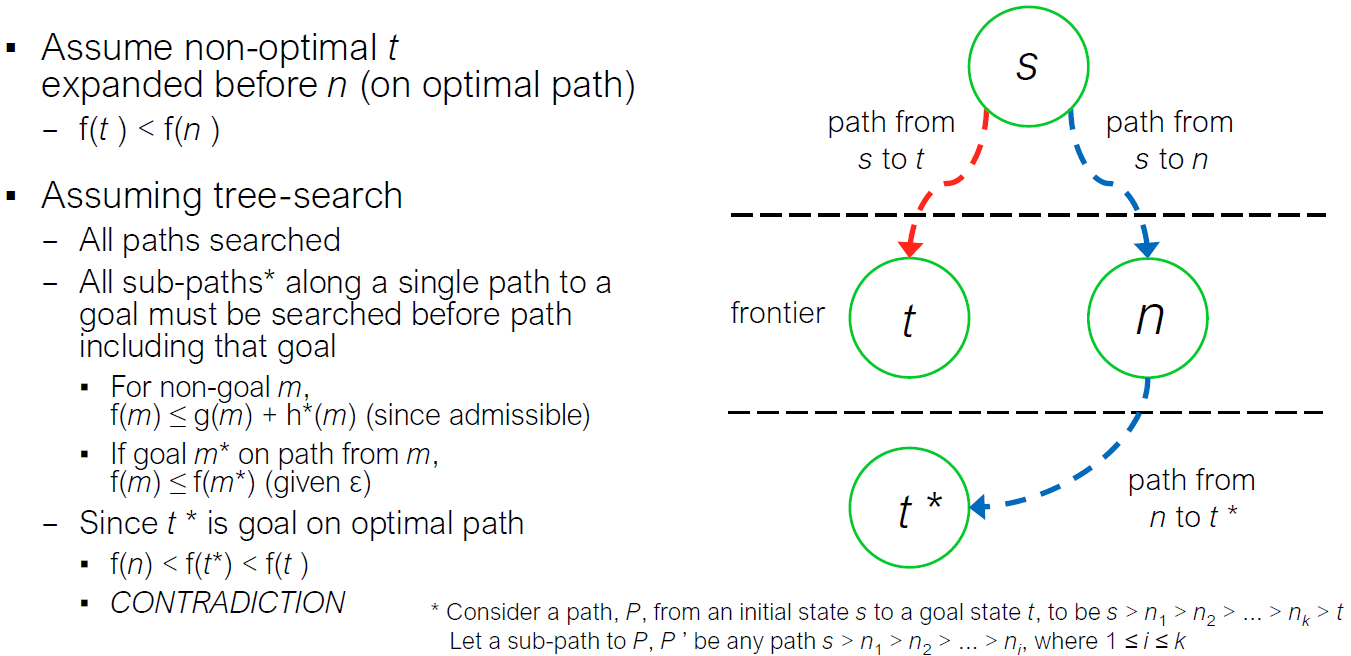
\includegraphics[width=0.7\columnwidth]{a-star-optimality}
  \end{center}
  \subsection{Why dominant heuristic is more efficient?}
  \begin{center}
  	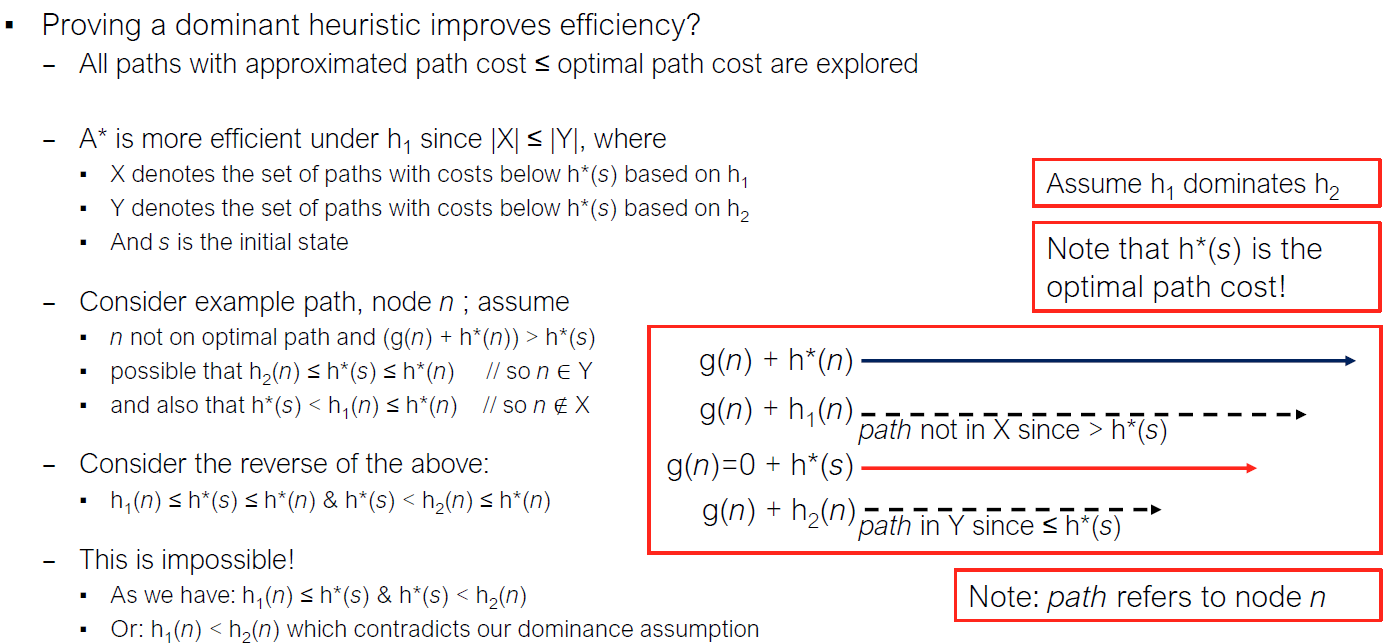
\includegraphics[width=0.7\columnwidth]{dominant-heuristic-efficiency}
  \end{center}
  \subsection{Why UCS time and space complexity is $O(b^{1+\left\lfloor\frac{C^*}{\epsilon}\right\rfloor})$}
  \begin{center}
	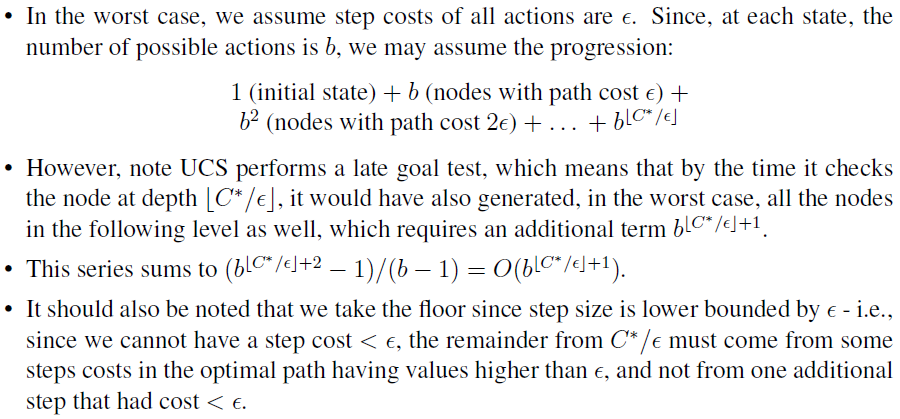
\includegraphics[width=0.7\columnwidth]{ucs-time-space-usage}
  \end{center}
  \subsection{Why deterministic search algo will search entire state space}
  \begin{itemize}
  	\item Idea is that it is possible to randomly pick a goal node $g_1$, run the algo and if it doesn't search the entire tree, pick another goal node $g_2$ that is in the unexplored set when $g_1$ is used
  	\item Can keep repeating these steps to force algo to search entire tree since it is a deterministic algorithm
  \end{itemize}
  \section{Miscellaneous}
  \subsection{Episodic vs Sequential}
  In most cases, when a human tries to solve a puzzle for e.g. Sudoku, the actions themselves are considered sequential. However, in the case of an intelligent agent, it would plan all the moves ahead. This makes the intelligent agent actions "episodic" where each action is the entire plan to solve one case of the maze.
  \subsection{Defaults for Graph Search}
  \begin{itemize}
  	\item All default to graph search V1 unless otherwise stated
  	\item BFS defaults to early goal test (stop when goal is found)
  \end{itemize}
  \subsection{Calculating Effective Branching Factor of Heuristics}
  \begin{itemize}
  	\item Given empirical results of $N$ nodes explored and solution depth of $d$
  	\item Solve for $b^*$ using $N+1=((b^*)^{d+1})/((b^*)-1)$
  \end{itemize}
  \subsection{Calculating size of search tree}
  \begin{itemize}
  	\item Geometric series: $a+ar+ar^2+\cdots+ar^{p-1}=a(r^p-1)/(r-1)$
  	\item Size of search tree: $(r^p-1)/(r-1)$
  \end{itemize}
  \section{Counter Examples}
  \subsection{Non-Optimality under Graph Search V1}
  \begin{center}
  	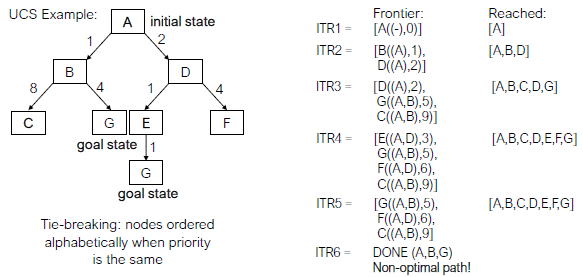
\includegraphics[width=0.7\columnwidth]{graph-v1-non-optimal}
  	\begin{center}
  		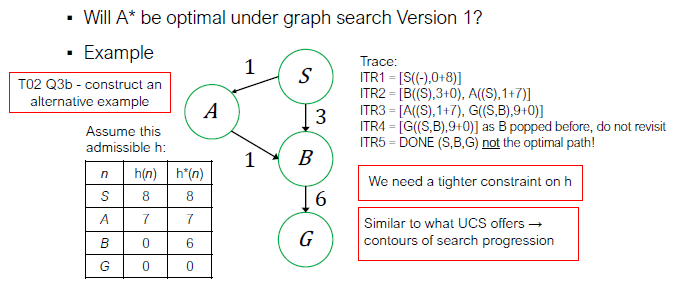
\includegraphics[width=0.7\columnwidth]{a-star-non-optimal}
  	\end{center}
  \end{center}
  \subsection{Non-Optimality using Greedy Best First Search}
  \begin{center}
  	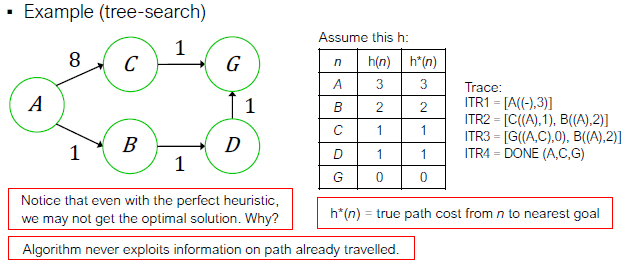
\includegraphics[width=0.7\columnwidth]{greedy-best-first-non-optimal}
  \end{center}
  \subsection{Non-Completeness using Greedy Best First Search}
  \begin{center}
  	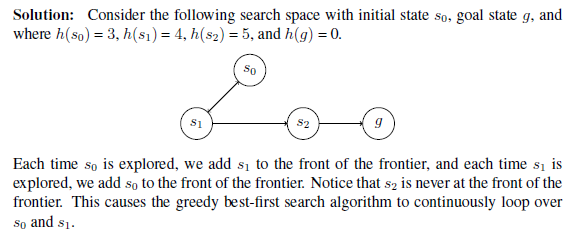
\includegraphics[width=0.7\columnwidth]{greedy-best-first-non-complete}
  \end{center}
  \subsection{Admissible but not consistent heuristic}
  \begin{center}
  	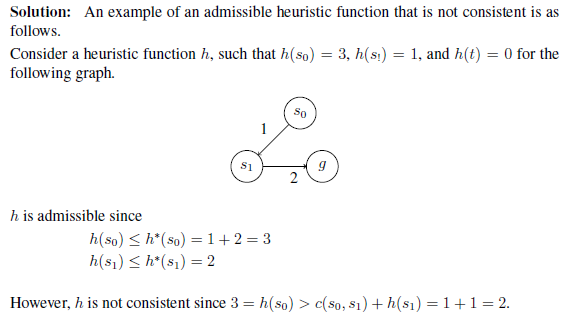
\includegraphics[width=0.7\columnwidth]{admissible-not-consistent}
  \end{center}
  \subsection{Non-Optimality of A$^*$ using consistent heuristic under Graph search V1}
  \begin{center}
  	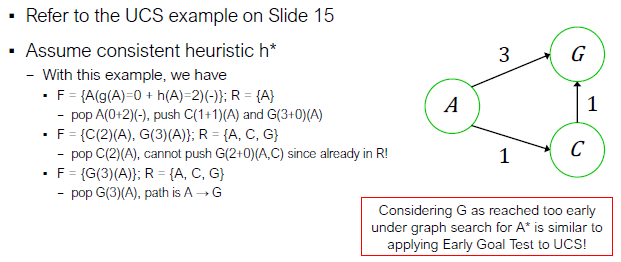
\includegraphics[width=0.7\columnwidth]{a-star-consistent-non-optimal}
  \end{center}
%  \section{Adversarial Search}
%  \begin{itemize}
%    \item 2 players, zero-sum game
%    \item \textbf{Game formulation}:
%          \begin{itemize}
%            \item $S_0$: The \textbf{initial state}
%            \item PLAYER(s): which player has the move in a state
%            \item ACTIONS(s): returns the set of legal moves in a state.
%            \item RESULT(s, a): The \textbf{transition model}, defines the result of a move
%            \item TERMINAL-TEST(s): A \textbf{terminal test}, true when game is over
%            \item UTILITY(s, p): A \textbf{utility function)}, defines final numeric value for a game that ends in terminal state $s$ for a player $p$
%          \end{itemize}
%  \end{itemize}
%  \subsection{Optimal Decisions in Games}
%  \begin{itemize}
%    \item \textbf{Winning} strategy for one player if for any strategy played by the other player, the game ended with the former as the winner. Similar for \textbf{non-losing} strategy.
%    \item \textbf{Nash Equilibrium} -- when players know the strategies of all opponents, no one wants to change their strategy.
%    \item \textbf{Subgame Perfect Nash Eq} -- every subgame is a \textbf{Nash Eq}
%  \end{itemize}
%  \subsection{Minimax}
%  \begin{itemize}
%    \item Optimal strategy can be determined from the \textbf{minimax value} of each node: utility (for MAX) of being in the state, assuming both players play optimally from there to the end of the game.
%    \item Minimax returns a subperfect Nash equilibrium
%    \item Minimax is \textbf{Complete} (with finite game tree), \textbf{Optimal}, \textbf{Time} $O(b^m)$, \textbf{Space} $O(bm)$
%  \end{itemize}
%  \subsection{$\alpha-\beta$ Pruning}
%  \begin{itemize}
%    \item MAX node n: $\alpha(n) = $ highest observed value found on path from n, initially $-\infty$
%    \item MIN node n: $\beta = $ lowest observed value found on path from n, initially $+\infty$
%    \item If a MIN node has value $v \leq \alpha(n)$, can prune
%    \item If a MAX node has value $v \geq \beta(n)$, can prune
%  \end{itemize}
%
%  \subsection{Imperfect Real-time Decisions}
%  \begin{itemize}
%    \item Although very large search space in typical games is pruned by $\alpha-\beta$ pruning, minimax still has to search all the way to the terminal states.
%    \item Replace utility function with heuristic \textbf{evaluation function} that estimates the position's utility, and replace the terminal test with a \textbf{cutoff test} that decides when to apply EVAL.
%  \end{itemize}
%  \subsection{Evaluation Functions}
%  \begin{itemize}
%    \item A mapping from game states to real values.
%    \item Should be cheap to compute; for non-terminal states, must be strongly correlated with actual chances of winning
%    \item Modern eval function: weighted sum of position features
%    \item Need not return actual expected values, just maintain relative order of states, typically from statistically probabilities
%  \end{itemize}
%  \subsection{Cutting off Search}
%  Stop after a certain depth, can be combined with iterative deepening
%
%  \section{Constraint Satisfaction Problems}
%  Consists of 3 components:
%  \begin{itemize}
%    \item $X$ is a set of variables, $\{X_1, ..., X_n\}$
%    \item $D$ is a set of domains, $\{D_1, ..., D_n\}$, one for each variable
%    \item $C$ is a set of constraints that specify allowable combinations of values
%  \end{itemize}
%  \subsection{Terminologies}
%  \begin{itemize}
%    \item \textbf{Consistent} assignment = does not vilate any constraints
%    \item \textbf{Complete} assignment = every variable is assigned
%    \item Goal: find a consistent and complete assignment
%    \item \textbf{Binary constraint} relates 2 variables
%    \item \textbf{Global constraint} involve an arbitrary number of variables
%    \item Every finite-domain constraint can be reduced to a set of binary constraints if enough auxiliary variables are introduced.
%    \item \textbf{Constraint graph}: nodes are variables, links are constraints
%  \end{itemize}
%  \subsection{Variants}
%  \begin{itemize}
%    \item Domain can be \textbf{discrete} (both \textbf{finite} and \textbf{infinite}) or \textbf{continuous}
%    \item For discrete, infinite domains, a \textbf{constraint language} must be used without enumeration
%  \end{itemize}
%  \subsection{Constraint propagation: Inference in CSP}
%  Try to infer illegal values for variables by performing constraint propagation
%
%  For unary constraints, node consistency; For binary constraints, arc consistency
%
%  \textbf{Arc Consistency} = a variable $X_i$ in CSP is arc-consistent with another variable $X_j$ if for every value in the current domain $D_i$ there is some value in the domain $D_j$ that satisfies the binary constraint on the arc $(X_i,X_j)$. A network is arc-consistent if every variable is arc-consistent with every other variable.
%  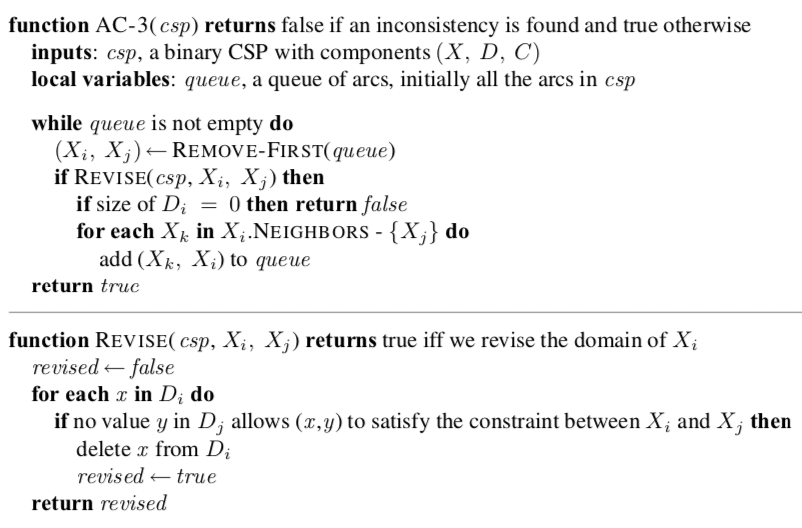
\includegraphics[width=\columnwidth]{ac-3}
%  \textbf{Time} $O(n^2d^3)$ where $n$ is number of vars, $d$ is max domain size
%
%  \textbf{$K$-consistency} = if, for any set of $k-1$ vars and for any consistent assignment to thsoe variables, a consistent value can always be assigned to any $k$-th var (arc-consistency is 2-consistency)
%
%  \subsection{Backtracking Search for CSPs}
%  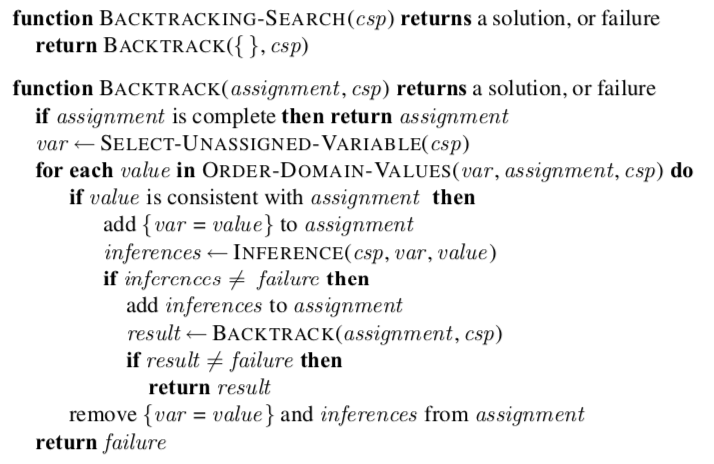
\includegraphics[width=\columnwidth]{backtrack}
%  \begin{itemize}
%    \item Better an just doing search, because CSPs are \textbf{commutative}
%    \item DFS that chooses values for one variable at a time, and backtracks when a var has no legal values left to assign.
%    \item For SELECT-UNASSIGNED-VARIABLE: use \textbf{Most Constrained Variable} choose the var with fewest legal values (Minimum Remaining Values (MRV) heuristic)
%    \item Once a variable is selected, to decide the order to examine its values, use \textbf{Least Constraining Value} heuristic: prefer value that rules out the fewest choices for the neighbouring variables in the constraint graph
%  \end{itemize}
%  \subsection{Local Search for CSPs}
%  \begin{itemize}
%    \item Similar to hill-climbing, but instead with complete states, allow states that violate constraints, then reassign variable values
%    \item In choosing a new value for a variable, herustic: select the value that results in the minimum number of conflicts with other variables
%  \end{itemize}
%  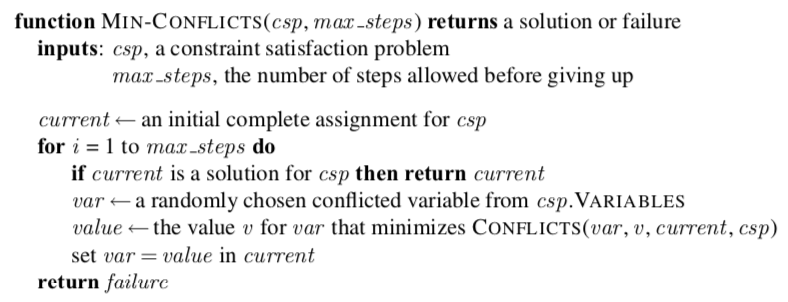
\includegraphics[width=\columnwidth]{min-conflict}
%  \subsection{The structure of problems}
%  \begin{itemize}
%    \item Theorem: if CSP constraint graph (with binary constraints) is a \textbf{tree}, then we can compute a satisfying assignment (or determine one does not exist) in $O(nd^2)$ time (no need to backtrack)
%    \item Proof: Pick any variable to be the root of tree, and choose an ordering of vars such that each var appears after its parent in the tree (Toposort: $O(n)$, each of which must compare up to $d$ possible domain values for the two variables)
%  \end{itemize}
\end{multicols*}
\end{document}
